\section{\acrshort{ddr}}
\subsection{Justification}
After implementing and validating a multicore and referee design, the next step that we faced was replacing the \textit{fake} memory with the \gls{fpga}'s \gls{ddr}.

As mentioned in Section \ref{sec:fpga}, \gls{sp7} has an integrated \gls{ddr} memory of 4 Gb.
We wanted to connect our current dual-core \gls{rtl} to \gls{ddr} since memory was a one with dummy cycles to simulate memory delay. 
So, we would have not to simulate a memory, but to deal with a real one.


\subsection{Xilinx \acrshort{ip}}
Xilinx provides a \glspl{ip}, which are validated \gls{rtl} codes that ease the usage of a certain component from the \gls{fpga}. 
Usually, they implement the \gls{phy}, hiding the complexity and the specific implementation details of the component, and provide an standard interface to the programmer. 
This is very usefull because the \gls{phy} of a component can change from one \gls{fpga} to another, so having an standar user interface allows programmers to not worry that much when porting a design from one \gls{fpga} to another, which it is usually a not trivial process.

The \gls{ip} used for the \gls{ddr} is: \gls{mig} \cite{mig}.
This \gls{ip} is a controller and implementation of the \gls{phy} for interfacing user designs and provides an \gls{axi} slave interface.
Therefore, the chain is: an user design connected via \gls{axi} to the \gls{ddr} device.

\subsubsection{\acrshort{axi} protocol}
\acrlong{axi} is an standard industry protocol to connect different components in order to exchange data.
It is usually used as an information exchange protocol between logic blocks inside a complex digital circuit.
The \gls{axi} interface requieres a low number of resources and provides a great uniderectional data transfer bandwidth \cite{axi}.

We can see in Figure \ref{fig:axi} the \gls{axi} handshake. %with the minimum signals, more can be added to provide more information.
Data (\texttt{information}) won't be transmited until the sender has valid data (\texttt{tvalid}) and the receiver is ready (\texttt{tready}).
It is composed by a master interface and a slave interface.

\begin{figure}
    \centering
    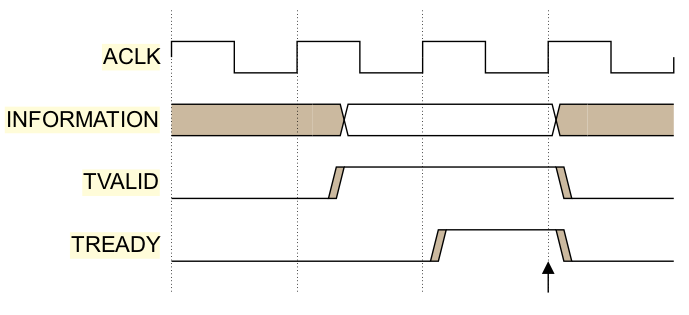
\includegraphics[width=0.7\textwidth]{../presentation/images/axi.png}
    \label{fig:axi}
    \caption{\gls{axi} handshake.}
\end{figure}

Information can be composed by many signal, the \texttt{data} one is the minimum one that has to be included.
Other signals can be added to \gls{axi} transactions in order to codify other information, such as the address.

\subsubsection{\acrshort{mig}}
As mentioned before, \gls{mig} provides an \gls{axi} interface to the programmer and is a customizable \gls{ip}. 
The most relevant options are the ones related to the \gls{axi} protocol, since they affect the \gls{rtl} design.
\begin{itemize}
    \item \texttt{ADDR\_WIDTH}: \\
        \gls{axi} address width for the slave and master interfaces. \\
        Options: up to 32 bits.
        
    \item \texttt{DATA\_WIDTH}: \\
        Width of the \gls{axi} read and write data for the slave and master interfaces. \\
        Options: 32, 64, 128, 256 bits.
\end{itemize}

The widths chosen are 32 bits for both options.

The \gls{mig} interface is the one that can be seen in Figure \ref{fig:mig}.
On the left side, there is the \gls{axi} interface to be connected with the user app. The left arrows indicate an input signal, and the right arrows an output.
On the right side, there is inputs/ouputs for the \gls{ddr} which are connected to the \gls{ddr} \gls{fpga}'s pins.

\begin{figure}
    \centering
    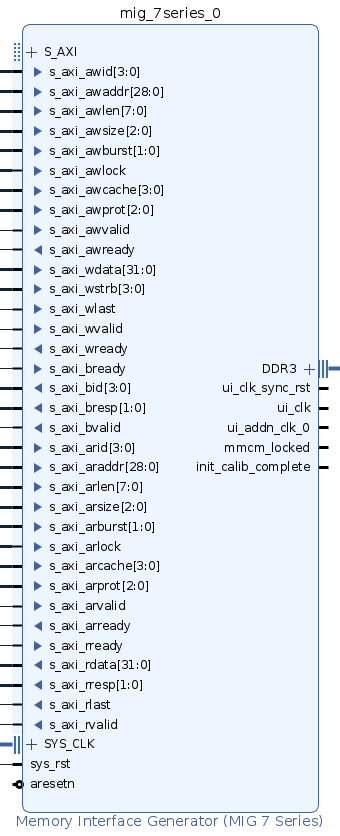
\includegraphics[width=0.55\textwidth]{img/mig_interface.png}
    \caption{\gls{mig} interface.}
    \label{fig:mig}
\end{figure}

\subsection{Implementation}
We implemented a \textit{bridge} to connect the \textit{referee} and the \gls{mig}.
It receives the transactions from the referee and refactors them into appropiated signals that the \gls{ddr} \gls{ip} needs. Also, a fine state machine was used to control the flow of the signals.

Therefore, the \gls{rtl} processor was modified in order to extract \gls{axi}'s \gls{mig} signals needed. 
The result is the block design that can be seen in Figure \ref{fig:bd_mig}, where our processors is connected to \gls{mig}.

    \begin{figure}
        \hspace{-3cm}
        \centering
        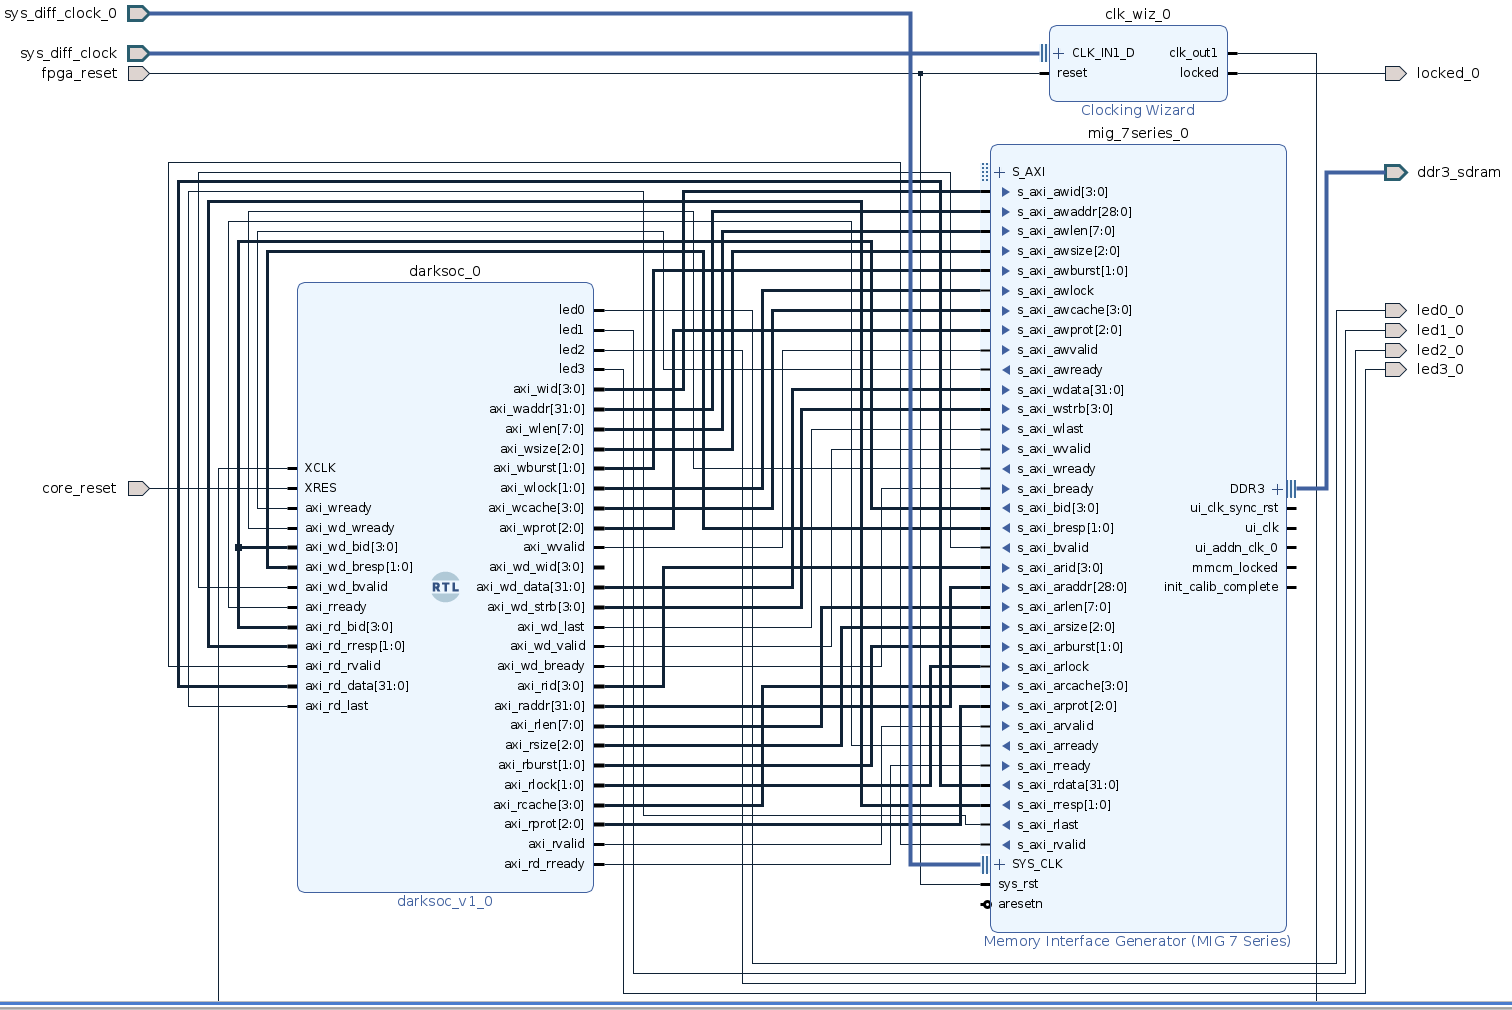
\includegraphics[width=1.2\textwidth]{../presentation/images/bd_ddr.png}
        \caption{Block design with \gls{mig}.}
        \label{fig:bd_mig}
    \end{figure}

\subsection{Validation}
The first validation step was with the Vivado simulator. 
\gls{mig} allows the simulation of the user app (our \gls{rtl} dual-core) and the \gls{ip} itself.

We adapted the testbench provided by Xilinx to connect our dual core. 
We ran the simulation and we detected that it was not simulating anything.
Some signals from the default waveform (the one provided in first intance by the \gls{ip} simulation) had a \texttt{Z} value, which means that they were not connected well.

We could not debbug the testbench in time.
The \gls{mig} testbench is a complex one, since it has to simulate the \gls{ddr}'s \gls{phy}, which is a tricky flow.

So, we could not proceed with the validation via simulation, and nor within the \gls{fpga}.

